\documentclass[a4paper,12pt]{article}
\usepackage[top = 2.5cm, bottom = 2.5cm, left = 2.5cm, right = 2.5cm]{geometry}
\usepackage[T1]{fontenc}
\usepackage[utf8]{inputenc}
\usepackage{multirow} 
\usepackage{booktabs} 
\usepackage{graphicx}
\usepackage{tikz}
\usepackage[spanish]{babel}
\usepackage{setspace}
\setlength{\parindent}{0in}
\usepackage{float}
\usepackage{fancyhdr}
\usepackage{amsmath}
\usepackage{amssymb}
\usepackage{amsthm}
\usepackage{natbib}
\usepackage{graphicx}
\usepackage{subcaption}
\usepackage{booktabs}
\usepackage{etoolbox}
\usepackage{apalike}
\usepackage{minibox}
\usepackage{hyperref}
\usepackage{xcolor}
\usepackage{tcolorbox}
\AtBeginEnvironment{align}{\setcounter{equation}{0}}
\newenvironment{solution}
  {\renewcommand\qedsymbol{$\square$}\begin{proof}[\textcolor{blue}{Solución}]}
  {\end{proof}}

\pagestyle{fancy}

\fancyhf{}

\lhead{\footnotesize Matemática Discreta - }
\rhead{\footnotesize  Rudik Roberto Rompich}
\cfoot{\footnotesize \thepage}

\begin{document}
    \thispagestyle{empty} 
    \begin{tabular}{p{15.5cm}}
    \begin{tabbing}
    \textbf{Universidad del Valle de Guatemala} \\
    Departamento de Matemática\\
    Licenciatura en Matemática Aplicada\\\\
   \textbf{Estudiante:} Rudik Roberto Rompich\\
   \textbf{E-mail:} \textcolor{blue}{ \href{mailto:rom19857@uvg.edu.gt}{rom19857@uvg.edu.gt}}\\
   \textbf{Carné:} 19857
    \end{tabbing}
    \begin{center}
        MM2015 - Matemática Discreta - Catedrático: Mario Castillo\\
        \today
    \end{center}\\
    \hline
    \\
    \end{tabular} 
    \vspace*{0.3cm} 
    \begin{center} 
    {\Large \bf Tarea 3
} 
        \vspace{2mm}
    \end{center}
    \vspace{0.4cm}
    %---------------------------
%\begin{tcolorbox}[colback=gray!15,colframe=black!1!black,title=A nice heading]
%\end{tcolorbox}

%\fbox{lol}

%---------------------------
\section{Problema 1}
Encuentre dos elementos no comparables en cada uno de los siguientes \textit{poset}:
\begin{enumerate}
    \item $(\mathcal{P}(\{0,1,2\}),\subseteq)$
    \begin{solution}Elementos:
    \begin{enumerate}
        \item $\{1\}\not\subseteq \{2\}$
        \item $ \{0\}\not\subseteq \{1,2\}$
    \end{enumerate}
    \end{solution}
    \item $(\{1,2,4,6,8\},|)$
    \begin{solution} Elementos:
    \begin{enumerate}
        \item 4 no es divisible dentro de 6.
        \item 6 no es divisible dentro de 8. 
    \end{enumerate}
    \end{solution}
\end{enumerate}

%----------------------------
\section{Problema 2}
Dibuje el diagrama de Hasse de la relación de divisibilidad en el conjuto: 
$$\{2,3,5,10,11,15,25\}$$
\begin{solution}
    Se determinan las parejas:
    $$(2,10),(3,15),(5,10),(5,15),(5,25)$$
    Entonces, se tiene: 
    \begin{center}
        

\tikzset{every picture/.style={line width=0.75pt}} %set default line width to 0.75pt        

\begin{tikzpicture}[x=0.75pt,y=0.75pt,yscale=-1,xscale=1]
%uncomment if require: \path (0,300); %set diagram left start at 0, and has height of 300

%Shape: Ellipse [id:dp7570623472300396] 
\draw   (283.42,154.35) .. controls (283.3,147.23) and (290.32,141.33) .. (299.09,141.18) .. controls (307.87,141.03) and (315.09,146.68) .. (315.21,153.81) .. controls (315.33,160.94) and (308.31,166.84) .. (299.54,166.99) .. controls (290.76,167.14) and (283.54,161.48) .. (283.42,154.35) -- cycle ;
%Straight Lines [id:da7554172544557495] 
\draw    (309.91,162.53) -- (308.73,163.91) ;
\draw [shift={(306.79,166.2)}, rotate = 310.36] [fill={rgb, 255:red, 0; green, 0; blue, 0 }  ][line width=0.08]  [draw opacity=0] (14.29,-6.86) -- (0,0) -- (14.29,6.86) -- (9.49,0) -- cycle    ;

%Shape: Ellipse [id:dp4503237325205852] 
\draw   (314.21,79.2) .. controls (314.16,86.33) and (307,92.05) .. (298.22,91.99) .. controls (289.44,91.92) and (282.37,86.09) .. (282.42,78.96) .. controls (282.47,71.84) and (289.63,66.11) .. (298.41,66.17) .. controls (307.19,66.24) and (314.26,72.07) .. (314.21,79.2) -- cycle ;
%Straight Lines [id:da41935664753500357] 
\draw    (287.93,70.38) -- (289.14,69.02) ;
\draw [shift={(291.14,66.79)}, rotate = 491.76] [fill={rgb, 255:red, 0; green, 0; blue, 0 }  ][line width=0.08]  [draw opacity=0] (14.29,-6.86) -- (0,0) -- (14.29,6.86) -- (9.49,0) -- cycle    ;

%Shape: Ellipse [id:dp5394406698129435] 
\draw   (238.21,81.2) .. controls (238.16,88.33) and (231,94.05) .. (222.22,93.99) .. controls (213.44,93.92) and (206.37,88.09) .. (206.42,80.96) .. controls (206.47,73.84) and (213.63,68.11) .. (222.41,68.17) .. controls (231.19,68.24) and (238.26,74.07) .. (238.21,81.2) -- cycle ;
%Straight Lines [id:da30806879052530456] 
\draw    (211.93,72.38) -- (213.14,71.02) ;
\draw [shift={(215.14,68.79)}, rotate = 491.76] [fill={rgb, 255:red, 0; green, 0; blue, 0 }  ][line width=0.08]  [draw opacity=0] (14.29,-6.86) -- (0,0) -- (14.29,6.86) -- (9.49,0) -- cycle    ;

%Shape: Ellipse [id:dp14347687268847487] 
\draw   (162.21,77.2) .. controls (162.16,84.33) and (155,90.05) .. (146.22,89.99) .. controls (137.44,89.92) and (130.37,84.09) .. (130.42,76.96) .. controls (130.47,69.84) and (137.63,64.11) .. (146.41,64.17) .. controls (155.19,64.24) and (162.26,70.07) .. (162.21,77.2) -- cycle ;
%Straight Lines [id:da17672091972634763] 
\draw    (135.93,68.38) -- (137.14,67.02) ;
\draw [shift={(139.14,64.79)}, rotate = 491.76] [fill={rgb, 255:red, 0; green, 0; blue, 0 }  ][line width=0.08]  [draw opacity=0] (14.29,-6.86) -- (0,0) -- (14.29,6.86) -- (9.49,0) -- cycle    ;

%Shape: Ellipse [id:dp4995620103872892] 
\draw   (97.21,123.2) .. controls (97.16,130.33) and (90,136.05) .. (81.22,135.99) .. controls (72.44,135.92) and (65.37,130.09) .. (65.42,122.96) .. controls (65.47,115.84) and (72.63,110.11) .. (81.41,110.17) .. controls (90.19,110.24) and (97.26,116.07) .. (97.21,123.2) -- cycle ;
%Straight Lines [id:da6935102563735467] 
\draw    (70.93,114.38) -- (72.14,113.02) ;
\draw [shift={(74.14,110.79)}, rotate = 491.76] [fill={rgb, 255:red, 0; green, 0; blue, 0 }  ][line width=0.08]  [draw opacity=0] (14.29,-6.86) -- (0,0) -- (14.29,6.86) -- (9.49,0) -- cycle    ;

%Shape: Ellipse [id:dp8678588878052144] 
\draw   (206.42,153.35) .. controls (206.3,146.23) and (213.32,140.33) .. (222.09,140.18) .. controls (230.87,140.03) and (238.09,145.68) .. (238.21,152.81) .. controls (238.33,159.94) and (231.31,165.84) .. (222.54,165.99) .. controls (213.76,166.14) and (206.54,160.48) .. (206.42,153.35) -- cycle ;
%Straight Lines [id:da5143139165904409] 
\draw    (232.91,161.53) -- (231.73,162.91) ;
\draw [shift={(229.79,165.2)}, rotate = 310.36] [fill={rgb, 255:red, 0; green, 0; blue, 0 }  ][line width=0.08]  [draw opacity=0] (14.29,-6.86) -- (0,0) -- (14.29,6.86) -- (9.49,0) -- cycle    ;

%Shape: Ellipse [id:dp12874959202918834] 
\draw   (132.19,151.59) .. controls (132.05,143.79) and (139.02,137.35) .. (147.76,137.2) .. controls (156.49,137.05) and (163.67,143.25) .. (163.81,151.05) .. controls (163.94,158.85) and (156.97,165.29) .. (148.24,165.44) .. controls (139.51,165.59) and (132.32,159.39) .. (132.19,151.59) -- cycle ;
%Straight Lines [id:da6872669009061414] 
\draw    (158.55,160.59) -- (157.29,162.22) ;
\draw [shift={(155.45,164.59)}, rotate = 307.67] [fill={rgb, 255:red, 0; green, 0; blue, 0 }  ][line width=0.08]  [draw opacity=0] (14.29,-6.86) -- (0,0) -- (14.29,6.86) -- (9.49,0) -- cycle    ;

%Shape: Ellipse [id:dp6089382434082271] 
\draw  [fill={rgb, 255:red, 208; green, 2; blue, 27 }  ,fill opacity=1 ] (288,140.21) .. controls (288,134.42) and (292.57,129.71) .. (298.21,129.71) .. controls (303.86,129.71) and (308.43,134.42) .. (308.43,140.21) .. controls (308.43,146.01) and (303.86,150.71) .. (298.21,150.71) .. controls (292.57,150.71) and (288,146.01) .. (288,140.21) -- cycle ;
%Shape: Ellipse [id:dp450092066763467] 
\draw  [fill={rgb, 255:red, 208; green, 2; blue, 27 }  ,fill opacity=1 ] (288,140.21) .. controls (288,134.42) and (292.57,129.71) .. (298.21,129.71) .. controls (303.86,129.71) and (308.43,134.42) .. (308.43,140.21) .. controls (308.43,146.01) and (303.86,150.71) .. (298.21,150.71) .. controls (292.57,150.71) and (288,146.01) .. (288,140.21) -- cycle ;
%Shape: Ellipse [id:dp2983624082990959] 
\draw  [fill={rgb, 255:red, 208; green, 2; blue, 27 }  ,fill opacity=1 ] (288,140.21) .. controls (288,134.42) and (292.57,129.71) .. (298.21,129.71) .. controls (303.86,129.71) and (308.43,134.42) .. (308.43,140.21) .. controls (308.43,146.01) and (303.86,150.71) .. (298.21,150.71) .. controls (292.57,150.71) and (288,146.01) .. (288,140.21) -- cycle ;
%Shape: Ellipse [id:dp6156794729448145] 
\draw  [fill={rgb, 255:red, 208; green, 2; blue, 27 }  ,fill opacity=1 ] (137,88.21) .. controls (137,82.42) and (141.57,77.71) .. (147.21,77.71) .. controls (152.86,77.71) and (157.43,82.42) .. (157.43,88.21) .. controls (157.43,94.01) and (152.86,98.71) .. (147.21,98.71) .. controls (141.57,98.71) and (137,94.01) .. (137,88.21) -- cycle ;
%Shape: Ellipse [id:dp03232105352911374] 
\draw  [fill={rgb, 255:red, 208; green, 2; blue, 27 }  ,fill opacity=1 ] (288,140.21) .. controls (288,134.42) and (292.57,129.71) .. (298.21,129.71) .. controls (303.86,129.71) and (308.43,134.42) .. (308.43,140.21) .. controls (308.43,146.01) and (303.86,150.71) .. (298.21,150.71) .. controls (292.57,150.71) and (288,146.01) .. (288,140.21) -- cycle ;
%Shape: Ellipse [id:dp6292281579283894] 
\draw  [fill={rgb, 255:red, 208; green, 2; blue, 27 }  ,fill opacity=1 ] (289,90.21) .. controls (289,84.42) and (293.57,79.71) .. (299.21,79.71) .. controls (304.86,79.71) and (309.43,84.42) .. (309.43,90.21) .. controls (309.43,96.01) and (304.86,100.71) .. (299.21,100.71) .. controls (293.57,100.71) and (289,96.01) .. (289,90.21) -- cycle ;
%Shape: Ellipse [id:dp7045525363557952] 
\draw  [fill={rgb, 255:red, 208; green, 2; blue, 27 }  ,fill opacity=1 ] (289,90.21) .. controls (289,84.42) and (293.57,79.71) .. (299.21,79.71) .. controls (304.86,79.71) and (309.43,84.42) .. (309.43,90.21) .. controls (309.43,96.01) and (304.86,100.71) .. (299.21,100.71) .. controls (293.57,100.71) and (289,96.01) .. (289,90.21) -- cycle ;
%Shape: Ellipse [id:dp3124371839153891] 
\draw  [fill={rgb, 255:red, 208; green, 2; blue, 27 }  ,fill opacity=1 ] (289,90.21) .. controls (289,84.42) and (293.57,79.71) .. (299.21,79.71) .. controls (304.86,79.71) and (309.43,84.42) .. (309.43,90.21) .. controls (309.43,96.01) and (304.86,100.71) .. (299.21,100.71) .. controls (293.57,100.71) and (289,96.01) .. (289,90.21) -- cycle ;
%Shape: Ellipse [id:dp5537826164972737] 
\draw  [fill={rgb, 255:red, 208; green, 2; blue, 27 }  ,fill opacity=1 ] (137,139.21) .. controls (137,133.42) and (141.57,128.71) .. (147.21,128.71) .. controls (152.86,128.71) and (157.43,133.42) .. (157.43,139.21) .. controls (157.43,145.01) and (152.86,149.71) .. (147.21,149.71) .. controls (141.57,149.71) and (137,145.01) .. (137,139.21) -- cycle ;
%Shape: Ellipse [id:dp1658082499735607] 
\draw  [fill={rgb, 255:red, 208; green, 2; blue, 27 }  ,fill opacity=1 ] (212,139.21) .. controls (212,133.42) and (216.57,128.71) .. (222.21,128.71) .. controls (227.86,128.71) and (232.43,133.42) .. (232.43,139.21) .. controls (232.43,145.01) and (227.86,149.71) .. (222.21,149.71) .. controls (216.57,149.71) and (212,145.01) .. (212,139.21) -- cycle ;
%Shape: Ellipse [id:dp10481694166686617] 
\draw  [fill={rgb, 255:red, 208; green, 2; blue, 27 }  ,fill opacity=1 ] (212,139.21) .. controls (212,133.42) and (216.57,128.71) .. (222.21,128.71) .. controls (227.86,128.71) and (232.43,133.42) .. (232.43,139.21) .. controls (232.43,145.01) and (227.86,149.71) .. (222.21,149.71) .. controls (216.57,149.71) and (212,145.01) .. (212,139.21) -- cycle ;
%Shape: Ellipse [id:dp4225408025712958] 
\draw  [fill={rgb, 255:red, 208; green, 2; blue, 27 }  ,fill opacity=1 ] (212,139.21) .. controls (212,133.42) and (216.57,128.71) .. (222.21,128.71) .. controls (227.86,128.71) and (232.43,133.42) .. (232.43,139.21) .. controls (232.43,145.01) and (227.86,149.71) .. (222.21,149.71) .. controls (216.57,149.71) and (212,145.01) .. (212,139.21) -- cycle ;
%Shape: Ellipse [id:dp7712968956685478] 
\draw  [fill={rgb, 255:red, 208; green, 2; blue, 27 }  ,fill opacity=1 ] (212,90.21) .. controls (212,84.42) and (216.57,79.71) .. (222.21,79.71) .. controls (227.86,79.71) and (232.43,84.42) .. (232.43,90.21) .. controls (232.43,96.01) and (227.86,100.71) .. (222.21,100.71) .. controls (216.57,100.71) and (212,96.01) .. (212,90.21) -- cycle ;
%Shape: Ellipse [id:dp9745586465759637] 
\draw  [fill={rgb, 255:red, 208; green, 2; blue, 27 }  ,fill opacity=1 ] (83,123.21) .. controls (83,117.42) and (87.57,112.71) .. (93.21,112.71) .. controls (98.86,112.71) and (103.43,117.42) .. (103.43,123.21) .. controls (103.43,129.01) and (98.86,133.71) .. (93.21,133.71) .. controls (87.57,133.71) and (83,129.01) .. (83,123.21) -- cycle ;
%Straight Lines [id:da6074586729898808] 
\draw    (222.21,128.71) -- (222.21,102.71) ;
\draw [shift={(222.21,100.71)}, rotate = 450] [color={rgb, 255:red, 0; green, 0; blue, 0 }  ][line width=0.75]    (10.93,-3.29) .. controls (6.95,-1.4) and (3.31,-0.3) .. (0,0) .. controls (3.31,0.3) and (6.95,1.4) .. (10.93,3.29)   ;
%Straight Lines [id:da8989824278578071] 
\draw    (298.21,129.71) -- (298.21,103.71) ;
\draw [shift={(298.21,101.71)}, rotate = 450] [color={rgb, 255:red, 0; green, 0; blue, 0 }  ][line width=0.75]    (10.93,-3.29) .. controls (6.95,-1.4) and (3.31,-0.3) .. (0,0) .. controls (3.31,0.3) and (6.95,1.4) .. (10.93,3.29)   ;
%Straight Lines [id:da804026890053836] 
\draw    (232.43,139.21) -- (290.8,97.87) ;
\draw [shift={(292.43,96.71)}, rotate = 504.69] [color={rgb, 255:red, 0; green, 0; blue, 0 }  ][line width=0.75]    (10.93,-3.29) .. controls (6.95,-1.4) and (3.31,-0.3) .. (0,0) .. controls (3.31,0.3) and (6.95,1.4) .. (10.93,3.29)   ;
%Straight Lines [id:da4586225854943642] 
\draw    (212.43,133.71) -- (156.11,97.79) ;
\draw [shift={(154.43,96.71)}, rotate = 392.53999999999996] [color={rgb, 255:red, 0; green, 0; blue, 0 }  ][line width=0.75]    (10.93,-3.29) .. controls (6.95,-1.4) and (3.31,-0.3) .. (0,0) .. controls (3.31,0.3) and (6.95,1.4) .. (10.93,3.29)   ;
%Straight Lines [id:da354302019933582] 
\draw    (147.21,128.71) -- (147.21,100.71) ;
\draw [shift={(147.21,98.71)}, rotate = 450] [color={rgb, 255:red, 0; green, 0; blue, 0 }  ][line width=0.75]    (10.93,-3.29) .. controls (6.95,-1.4) and (3.31,-0.3) .. (0,0) .. controls (3.31,0.3) and (6.95,1.4) .. (10.93,3.29)   ;

% Text Node
\draw (293.41,131.69) node [anchor=north west][inner sep=0.75pt]  [color={rgb, 255:red, 255; green, 255; blue, 255 }  ,opacity=1 ] [align=left] {2};
% Text Node
\draw (138.41,79.69) node [anchor=north west][inner sep=0.75pt]  [color={rgb, 255:red, 255; green, 255; blue, 255 }  ,opacity=1 ] [align=left] {15};
% Text Node
\draw (289.41,82.69) node [anchor=north west][inner sep=0.75pt]  [color={rgb, 255:red, 255; green, 255; blue, 255 }  ,opacity=1 ] [align=left] {10};
% Text Node
\draw (142.41,130.69) node [anchor=north west][inner sep=0.75pt]  [color={rgb, 255:red, 255; green, 255; blue, 255 }  ,opacity=1 ] [align=left] {3};
% Text Node
\draw (217.41,130.69) node [anchor=north west][inner sep=0.75pt]  [color={rgb, 255:red, 255; green, 255; blue, 255 }  ,opacity=1 ] [align=left] {5};
% Text Node
\draw (217.41,130.69) node [anchor=north west][inner sep=0.75pt]  [color={rgb, 255:red, 255; green, 255; blue, 255 }  ,opacity=1 ] [align=left] {5};
% Text Node
\draw (367.41,204.69) node [anchor=north west][inner sep=0.75pt]  [color={rgb, 255:red, 255; green, 255; blue, 255 }  ,opacity=1 ] [align=left] {5};
% Text Node
\draw (213.41,81.69) node [anchor=north west][inner sep=0.75pt]  [color={rgb, 255:red, 255; green, 255; blue, 255 }  ,opacity=1 ] [align=left] {25};
% Text Node
\draw (85.41,115.69) node [anchor=north west][inner sep=0.75pt]  [color={rgb, 255:red, 255; green, 255; blue, 255 }  ,opacity=1 ] [align=left] {11};
\end{tikzpicture}
    \end{center}
    Por lo cual, se tiene: 
    \begin{center}
        

\tikzset{every picture/.style={line width=0.75pt}} %set default line width to 0.75pt        

\begin{tikzpicture}[x=0.75pt,y=0.75pt,yscale=-1,xscale=1]
%uncomment if require: \path (0,300); %set diagram left start at 0, and has height of 300

%Shape: Ellipse [id:dp6089382434082271] 
\draw  [fill={rgb, 255:red, 208; green, 2; blue, 27 }  ,fill opacity=1 ] (288,140.21) .. controls (288,134.42) and (292.57,129.71) .. (298.21,129.71) .. controls (303.86,129.71) and (308.43,134.42) .. (308.43,140.21) .. controls (308.43,146.01) and (303.86,150.71) .. (298.21,150.71) .. controls (292.57,150.71) and (288,146.01) .. (288,140.21) -- cycle ;
%Shape: Ellipse [id:dp450092066763467] 
\draw  [fill={rgb, 255:red, 208; green, 2; blue, 27 }  ,fill opacity=1 ] (288,140.21) .. controls (288,134.42) and (292.57,129.71) .. (298.21,129.71) .. controls (303.86,129.71) and (308.43,134.42) .. (308.43,140.21) .. controls (308.43,146.01) and (303.86,150.71) .. (298.21,150.71) .. controls (292.57,150.71) and (288,146.01) .. (288,140.21) -- cycle ;
%Shape: Ellipse [id:dp2983624082990959] 
\draw  [fill={rgb, 255:red, 208; green, 2; blue, 27 }  ,fill opacity=1 ] (288,140.21) .. controls (288,134.42) and (292.57,129.71) .. (298.21,129.71) .. controls (303.86,129.71) and (308.43,134.42) .. (308.43,140.21) .. controls (308.43,146.01) and (303.86,150.71) .. (298.21,150.71) .. controls (292.57,150.71) and (288,146.01) .. (288,140.21) -- cycle ;
%Shape: Ellipse [id:dp6156794729448145] 
\draw  [fill={rgb, 255:red, 208; green, 2; blue, 27 }  ,fill opacity=1 ] (137,88.21) .. controls (137,82.42) and (141.57,77.71) .. (147.21,77.71) .. controls (152.86,77.71) and (157.43,82.42) .. (157.43,88.21) .. controls (157.43,94.01) and (152.86,98.71) .. (147.21,98.71) .. controls (141.57,98.71) and (137,94.01) .. (137,88.21) -- cycle ;
%Shape: Ellipse [id:dp03232105352911374] 
\draw  [fill={rgb, 255:red, 208; green, 2; blue, 27 }  ,fill opacity=1 ] (288,140.21) .. controls (288,134.42) and (292.57,129.71) .. (298.21,129.71) .. controls (303.86,129.71) and (308.43,134.42) .. (308.43,140.21) .. controls (308.43,146.01) and (303.86,150.71) .. (298.21,150.71) .. controls (292.57,150.71) and (288,146.01) .. (288,140.21) -- cycle ;
%Shape: Ellipse [id:dp6292281579283894] 
\draw  [fill={rgb, 255:red, 208; green, 2; blue, 27 }  ,fill opacity=1 ] (289,90.21) .. controls (289,84.42) and (293.57,79.71) .. (299.21,79.71) .. controls (304.86,79.71) and (309.43,84.42) .. (309.43,90.21) .. controls (309.43,96.01) and (304.86,100.71) .. (299.21,100.71) .. controls (293.57,100.71) and (289,96.01) .. (289,90.21) -- cycle ;
%Shape: Ellipse [id:dp7045525363557952] 
\draw  [fill={rgb, 255:red, 208; green, 2; blue, 27 }  ,fill opacity=1 ] (289,90.21) .. controls (289,84.42) and (293.57,79.71) .. (299.21,79.71) .. controls (304.86,79.71) and (309.43,84.42) .. (309.43,90.21) .. controls (309.43,96.01) and (304.86,100.71) .. (299.21,100.71) .. controls (293.57,100.71) and (289,96.01) .. (289,90.21) -- cycle ;
%Shape: Ellipse [id:dp3124371839153891] 
\draw  [fill={rgb, 255:red, 208; green, 2; blue, 27 }  ,fill opacity=1 ] (289,90.21) .. controls (289,84.42) and (293.57,79.71) .. (299.21,79.71) .. controls (304.86,79.71) and (309.43,84.42) .. (309.43,90.21) .. controls (309.43,96.01) and (304.86,100.71) .. (299.21,100.71) .. controls (293.57,100.71) and (289,96.01) .. (289,90.21) -- cycle ;
%Shape: Ellipse [id:dp5537826164972737] 
\draw  [fill={rgb, 255:red, 208; green, 2; blue, 27 }  ,fill opacity=1 ] (137,139.21) .. controls (137,133.42) and (141.57,128.71) .. (147.21,128.71) .. controls (152.86,128.71) and (157.43,133.42) .. (157.43,139.21) .. controls (157.43,145.01) and (152.86,149.71) .. (147.21,149.71) .. controls (141.57,149.71) and (137,145.01) .. (137,139.21) -- cycle ;
%Shape: Ellipse [id:dp1658082499735607] 
\draw  [fill={rgb, 255:red, 208; green, 2; blue, 27 }  ,fill opacity=1 ] (212,139.21) .. controls (212,133.42) and (216.57,128.71) .. (222.21,128.71) .. controls (227.86,128.71) and (232.43,133.42) .. (232.43,139.21) .. controls (232.43,145.01) and (227.86,149.71) .. (222.21,149.71) .. controls (216.57,149.71) and (212,145.01) .. (212,139.21) -- cycle ;
%Shape: Ellipse [id:dp10481694166686617] 
\draw  [fill={rgb, 255:red, 208; green, 2; blue, 27 }  ,fill opacity=1 ] (212,139.21) .. controls (212,133.42) and (216.57,128.71) .. (222.21,128.71) .. controls (227.86,128.71) and (232.43,133.42) .. (232.43,139.21) .. controls (232.43,145.01) and (227.86,149.71) .. (222.21,149.71) .. controls (216.57,149.71) and (212,145.01) .. (212,139.21) -- cycle ;
%Shape: Ellipse [id:dp4225408025712958] 
\draw  [fill={rgb, 255:red, 208; green, 2; blue, 27 }  ,fill opacity=1 ] (212,139.21) .. controls (212,133.42) and (216.57,128.71) .. (222.21,128.71) .. controls (227.86,128.71) and (232.43,133.42) .. (232.43,139.21) .. controls (232.43,145.01) and (227.86,149.71) .. (222.21,149.71) .. controls (216.57,149.71) and (212,145.01) .. (212,139.21) -- cycle ;
%Shape: Ellipse [id:dp7712968956685478] 
\draw  [fill={rgb, 255:red, 208; green, 2; blue, 27 }  ,fill opacity=1 ] (212,90.21) .. controls (212,84.42) and (216.57,79.71) .. (222.21,79.71) .. controls (227.86,79.71) and (232.43,84.42) .. (232.43,90.21) .. controls (232.43,96.01) and (227.86,100.71) .. (222.21,100.71) .. controls (216.57,100.71) and (212,96.01) .. (212,90.21) -- cycle ;
%Shape: Ellipse [id:dp9745586465759637] 
\draw  [fill={rgb, 255:red, 208; green, 2; blue, 27 }  ,fill opacity=1 ] (83,123.21) .. controls (83,117.42) and (87.57,112.71) .. (93.21,112.71) .. controls (98.86,112.71) and (103.43,117.42) .. (103.43,123.21) .. controls (103.43,129.01) and (98.86,133.71) .. (93.21,133.71) .. controls (87.57,133.71) and (83,129.01) .. (83,123.21) -- cycle ;
%Straight Lines [id:da6074586729898808] 
\draw    (222.21,128.71) -- (222.21,102.71) ;
\draw [shift={(222.21,100.71)}, rotate = 450] [color={rgb, 255:red, 0; green, 0; blue, 0 }  ][line width=0.75]    (10.93,-3.29) .. controls (6.95,-1.4) and (3.31,-0.3) .. (0,0) .. controls (3.31,0.3) and (6.95,1.4) .. (10.93,3.29)   ;
%Straight Lines [id:da8989824278578071] 
\draw    (298.21,129.71) -- (298.21,103.71) ;
\draw [shift={(298.21,101.71)}, rotate = 450] [color={rgb, 255:red, 0; green, 0; blue, 0 }  ][line width=0.75]    (10.93,-3.29) .. controls (6.95,-1.4) and (3.31,-0.3) .. (0,0) .. controls (3.31,0.3) and (6.95,1.4) .. (10.93,3.29)   ;
%Straight Lines [id:da804026890053836] 
\draw    (232.43,139.21) -- (290.8,97.87) ;
\draw [shift={(292.43,96.71)}, rotate = 504.69] [color={rgb, 255:red, 0; green, 0; blue, 0 }  ][line width=0.75]    (10.93,-3.29) .. controls (6.95,-1.4) and (3.31,-0.3) .. (0,0) .. controls (3.31,0.3) and (6.95,1.4) .. (10.93,3.29)   ;
%Straight Lines [id:da4586225854943642] 
\draw    (212.43,133.71) -- (156.11,97.79) ;
\draw [shift={(154.43,96.71)}, rotate = 392.53999999999996] [color={rgb, 255:red, 0; green, 0; blue, 0 }  ][line width=0.75]    (10.93,-3.29) .. controls (6.95,-1.4) and (3.31,-0.3) .. (0,0) .. controls (3.31,0.3) and (6.95,1.4) .. (10.93,3.29)   ;
%Straight Lines [id:da354302019933582] 
\draw    (147.21,128.71) -- (147.21,100.71) ;
\draw [shift={(147.21,98.71)}, rotate = 450] [color={rgb, 255:red, 0; green, 0; blue, 0 }  ][line width=0.75]    (10.93,-3.29) .. controls (6.95,-1.4) and (3.31,-0.3) .. (0,0) .. controls (3.31,0.3) and (6.95,1.4) .. (10.93,3.29)   ;

% Text Node
\draw (293.41,131.69) node [anchor=north west][inner sep=0.75pt]  [color={rgb, 255:red, 255; green, 255; blue, 255 }  ,opacity=1 ] [align=left] {2};
% Text Node
\draw (138.41,79.69) node [anchor=north west][inner sep=0.75pt]  [color={rgb, 255:red, 255; green, 255; blue, 255 }  ,opacity=1 ] [align=left] {15};
% Text Node
\draw (289.41,82.69) node [anchor=north west][inner sep=0.75pt]  [color={rgb, 255:red, 255; green, 255; blue, 255 }  ,opacity=1 ] [align=left] {10};
% Text Node
\draw (142.41,130.69) node [anchor=north west][inner sep=0.75pt]  [color={rgb, 255:red, 255; green, 255; blue, 255 }  ,opacity=1 ] [align=left] {3};
% Text Node
\draw (217.41,130.69) node [anchor=north west][inner sep=0.75pt]  [color={rgb, 255:red, 255; green, 255; blue, 255 }  ,opacity=1 ] [align=left] {5};
% Text Node
\draw (217.41,130.69) node [anchor=north west][inner sep=0.75pt]  [color={rgb, 255:red, 255; green, 255; blue, 255 }  ,opacity=1 ] [align=left] {5};
% Text Node
\draw (367.41,204.69) node [anchor=north west][inner sep=0.75pt]  [color={rgb, 255:red, 255; green, 255; blue, 255 }  ,opacity=1 ] [align=left] {5};
% Text Node
\draw (213.41,81.69) node [anchor=north west][inner sep=0.75pt]  [color={rgb, 255:red, 255; green, 255; blue, 255 }  ,opacity=1 ] [align=left] {25};
% Text Node
\draw (85.41,115.69) node [anchor=north west][inner sep=0.75pt]  [color={rgb, 255:red, 255; green, 255; blue, 255 }  ,opacity=1 ] [align=left] {11};


\end{tikzpicture}
    \end{center}
    Finalmente, el diagrama de Hess: 
    \begin{center}
        

\tikzset{every picture/.style={line width=0.75pt}} %set default line width to 0.75pt        

\begin{tikzpicture}[x=0.75pt,y=0.75pt,yscale=-1,xscale=1]
%uncomment if require: \path (0,300); %set diagram left start at 0, and has height of 300

%Shape: Ellipse [id:dp6089382434082271] 
\draw  [fill={rgb, 255:red, 208; green, 2; blue, 27 }  ,fill opacity=1 ] (288,140.21) .. controls (288,134.42) and (292.57,129.71) .. (298.21,129.71) .. controls (303.86,129.71) and (308.43,134.42) .. (308.43,140.21) .. controls (308.43,146.01) and (303.86,150.71) .. (298.21,150.71) .. controls (292.57,150.71) and (288,146.01) .. (288,140.21) -- cycle ;
%Shape: Ellipse [id:dp450092066763467] 
\draw  [fill={rgb, 255:red, 208; green, 2; blue, 27 }  ,fill opacity=1 ] (288,140.21) .. controls (288,134.42) and (292.57,129.71) .. (298.21,129.71) .. controls (303.86,129.71) and (308.43,134.42) .. (308.43,140.21) .. controls (308.43,146.01) and (303.86,150.71) .. (298.21,150.71) .. controls (292.57,150.71) and (288,146.01) .. (288,140.21) -- cycle ;
%Shape: Ellipse [id:dp2983624082990959] 
\draw  [fill={rgb, 255:red, 208; green, 2; blue, 27 }  ,fill opacity=1 ] (288,140.21) .. controls (288,134.42) and (292.57,129.71) .. (298.21,129.71) .. controls (303.86,129.71) and (308.43,134.42) .. (308.43,140.21) .. controls (308.43,146.01) and (303.86,150.71) .. (298.21,150.71) .. controls (292.57,150.71) and (288,146.01) .. (288,140.21) -- cycle ;
%Shape: Ellipse [id:dp6156794729448145] 
\draw  [fill={rgb, 255:red, 208; green, 2; blue, 27 }  ,fill opacity=1 ] (137,88.21) .. controls (137,82.42) and (141.57,77.71) .. (147.21,77.71) .. controls (152.86,77.71) and (157.43,82.42) .. (157.43,88.21) .. controls (157.43,94.01) and (152.86,98.71) .. (147.21,98.71) .. controls (141.57,98.71) and (137,94.01) .. (137,88.21) -- cycle ;
%Shape: Ellipse [id:dp03232105352911374] 
\draw  [fill={rgb, 255:red, 208; green, 2; blue, 27 }  ,fill opacity=1 ] (288,140.21) .. controls (288,134.42) and (292.57,129.71) .. (298.21,129.71) .. controls (303.86,129.71) and (308.43,134.42) .. (308.43,140.21) .. controls (308.43,146.01) and (303.86,150.71) .. (298.21,150.71) .. controls (292.57,150.71) and (288,146.01) .. (288,140.21) -- cycle ;
%Shape: Ellipse [id:dp6292281579283894] 
\draw  [fill={rgb, 255:red, 208; green, 2; blue, 27 }  ,fill opacity=1 ] (289,90.21) .. controls (289,84.42) and (293.57,79.71) .. (299.21,79.71) .. controls (304.86,79.71) and (309.43,84.42) .. (309.43,90.21) .. controls (309.43,96.01) and (304.86,100.71) .. (299.21,100.71) .. controls (293.57,100.71) and (289,96.01) .. (289,90.21) -- cycle ;
%Shape: Ellipse [id:dp7045525363557952] 
\draw  [fill={rgb, 255:red, 208; green, 2; blue, 27 }  ,fill opacity=1 ] (289,90.21) .. controls (289,84.42) and (293.57,79.71) .. (299.21,79.71) .. controls (304.86,79.71) and (309.43,84.42) .. (309.43,90.21) .. controls (309.43,96.01) and (304.86,100.71) .. (299.21,100.71) .. controls (293.57,100.71) and (289,96.01) .. (289,90.21) -- cycle ;
%Shape: Ellipse [id:dp3124371839153891] 
\draw  [fill={rgb, 255:red, 208; green, 2; blue, 27 }  ,fill opacity=1 ] (289,90.21) .. controls (289,84.42) and (293.57,79.71) .. (299.21,79.71) .. controls (304.86,79.71) and (309.43,84.42) .. (309.43,90.21) .. controls (309.43,96.01) and (304.86,100.71) .. (299.21,100.71) .. controls (293.57,100.71) and (289,96.01) .. (289,90.21) -- cycle ;
%Shape: Ellipse [id:dp5537826164972737] 
\draw  [fill={rgb, 255:red, 208; green, 2; blue, 27 }  ,fill opacity=1 ] (137,139.21) .. controls (137,133.42) and (141.57,128.71) .. (147.21,128.71) .. controls (152.86,128.71) and (157.43,133.42) .. (157.43,139.21) .. controls (157.43,145.01) and (152.86,149.71) .. (147.21,149.71) .. controls (141.57,149.71) and (137,145.01) .. (137,139.21) -- cycle ;
%Shape: Ellipse [id:dp1658082499735607] 
\draw  [fill={rgb, 255:red, 208; green, 2; blue, 27 }  ,fill opacity=1 ] (212,139.21) .. controls (212,133.42) and (216.57,128.71) .. (222.21,128.71) .. controls (227.86,128.71) and (232.43,133.42) .. (232.43,139.21) .. controls (232.43,145.01) and (227.86,149.71) .. (222.21,149.71) .. controls (216.57,149.71) and (212,145.01) .. (212,139.21) -- cycle ;
%Shape: Ellipse [id:dp10481694166686617] 
\draw  [fill={rgb, 255:red, 208; green, 2; blue, 27 }  ,fill opacity=1 ] (212,139.21) .. controls (212,133.42) and (216.57,128.71) .. (222.21,128.71) .. controls (227.86,128.71) and (232.43,133.42) .. (232.43,139.21) .. controls (232.43,145.01) and (227.86,149.71) .. (222.21,149.71) .. controls (216.57,149.71) and (212,145.01) .. (212,139.21) -- cycle ;
%Shape: Ellipse [id:dp4225408025712958] 
\draw  [fill={rgb, 255:red, 208; green, 2; blue, 27 }  ,fill opacity=1 ] (212,139.21) .. controls (212,133.42) and (216.57,128.71) .. (222.21,128.71) .. controls (227.86,128.71) and (232.43,133.42) .. (232.43,139.21) .. controls (232.43,145.01) and (227.86,149.71) .. (222.21,149.71) .. controls (216.57,149.71) and (212,145.01) .. (212,139.21) -- cycle ;
%Shape: Ellipse [id:dp7712968956685478] 
\draw  [fill={rgb, 255:red, 208; green, 2; blue, 27 }  ,fill opacity=1 ] (212,90.21) .. controls (212,84.42) and (216.57,79.71) .. (222.21,79.71) .. controls (227.86,79.71) and (232.43,84.42) .. (232.43,90.21) .. controls (232.43,96.01) and (227.86,100.71) .. (222.21,100.71) .. controls (216.57,100.71) and (212,96.01) .. (212,90.21) -- cycle ;
%Shape: Ellipse [id:dp9745586465759637] 
\draw  [fill={rgb, 255:red, 208; green, 2; blue, 27 }  ,fill opacity=1 ] (83,123.21) .. controls (83,117.42) and (87.57,112.71) .. (93.21,112.71) .. controls (98.86,112.71) and (103.43,117.42) .. (103.43,123.21) .. controls (103.43,129.01) and (98.86,133.71) .. (93.21,133.71) .. controls (87.57,133.71) and (83,129.01) .. (83,123.21) -- cycle ;
%Straight Lines [id:da6074586729898808] 
\draw    (222.21,128.71) -- (222.21,100.71) ;
%Straight Lines [id:da8989824278578071] 
\draw    (298.21,129.71) -- (298.21,101.71) ;
%Straight Lines [id:da804026890053836] 
\draw    (232.43,139.21) -- (292.43,96.71) ;
%Straight Lines [id:da4586225854943642] 
\draw    (212.43,133.71) -- (154.43,96.71) ;
%Straight Lines [id:da354302019933582] 
\draw    (147.21,128.71) -- (147.21,98.71) ;

% Text Node
\draw (293.41,131.69) node [anchor=north west][inner sep=0.75pt]  [color={rgb, 255:red, 255; green, 255; blue, 255 }  ,opacity=1 ] [align=left] {2};
% Text Node
\draw (138.41,79.69) node [anchor=north west][inner sep=0.75pt]  [color={rgb, 255:red, 255; green, 255; blue, 255 }  ,opacity=1 ] [align=left] {15};
% Text Node
\draw (289.41,82.69) node [anchor=north west][inner sep=0.75pt]  [color={rgb, 255:red, 255; green, 255; blue, 255 }  ,opacity=1 ] [align=left] {10};
% Text Node
\draw (142.41,130.69) node [anchor=north west][inner sep=0.75pt]  [color={rgb, 255:red, 255; green, 255; blue, 255 }  ,opacity=1 ] [align=left] {3};
% Text Node
\draw (217.41,130.69) node [anchor=north west][inner sep=0.75pt]  [color={rgb, 255:red, 255; green, 255; blue, 255 }  ,opacity=1 ] [align=left] {5};
% Text Node
\draw (217.41,130.69) node [anchor=north west][inner sep=0.75pt]  [color={rgb, 255:red, 255; green, 255; blue, 255 }  ,opacity=1 ] [align=left] {5};
% Text Node
\draw (367.41,204.69) node [anchor=north west][inner sep=0.75pt]  [color={rgb, 255:red, 255; green, 255; blue, 255 }  ,opacity=1 ] [align=left] {5};
% Text Node
\draw (213.41,81.69) node [anchor=north west][inner sep=0.75pt]  [color={rgb, 255:red, 255; green, 255; blue, 255 }  ,opacity=1 ] [align=left] {25};
% Text Node
\draw (85.41,115.69) node [anchor=north west][inner sep=0.75pt]  [color={rgb, 255:red, 255; green, 255; blue, 255 }  ,opacity=1 ] [align=left] {11};


\end{tikzpicture}
    \end{center}
\end{solution}

%----------------------------
\section{Problema 3}
Enumere todos los pares ordenados de cada uno de los \textit{posets} cuyos diagramas de Hasse se muestran a continuación. 

\begin{enumerate}
    \item Diagrama 
    \begin{center}
        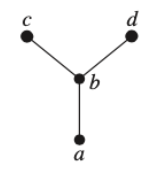
\includegraphics[scale=0.5]{Images/hasse1.png}
    \end{center}
    \begin{solution}
    $(a,a), (b,b), (c,c), (d,d), (a,b), (a,d), (b,d), (b,c), (a,c)$
    \end{solution}
    \item Diagrama
    \begin{center}
        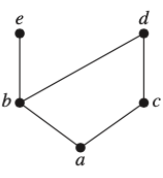
\includegraphics[scale=0.5]{Images/hasse2.png}
    \end{center}
    \begin{solution}
    $(a,c), (a,d), (a,b), (a,e), (c,d), (b,d), (b,e), (a,a), (b,b), (c,c),$\\$ (d,d), (e,e)$
    \end{solution}
    \item Diagrama
    \begin{center}
        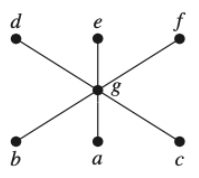
\includegraphics[scale=0.5]{Images/hasse3.png}
    \end{center}
    \begin{solution}
    $(b,g), (b,d), (b,e), (b,f), (a,g), (a,d),(a,e),(a,f), (c,g), (c,d),$\\$ (c,e), (c,f), (g,d),(g,e),(g,f), (a,a), (b,b), (c,c),(d,d), (e,e), (f,f), (g,g)$
    \end{solution}
\end{enumerate}

%----------------------------
\section{Problema 4}

Responda las siguientes preguntas acerca del conjunto parcialmente ordenado:
$$(\{3,5,9,15,24,45\}, |)$$
Se tiene: 
$$(3,9), (3,15), (3,24), (3,45), (5, 15), (5, 45), (9,45), (15, 45), $$
$$(3,3),(5,5),(9,9),(15,15),(24,24),(45,45)$$
Diagrama de Hess: 
\begin{center}
   

\tikzset{every picture/.style={line width=0.75pt}} %set default line width to 0.75pt        

\begin{tikzpicture}[x=0.75pt,y=0.75pt,yscale=-1,xscale=1]
%uncomment if require: \path (0,300); %set diagram left start at 0, and has height of 300

%Shape: Ellipse [id:dp07402318935785024] 
\draw  [fill={rgb, 255:red, 208; green, 2; blue, 27 }  ,fill opacity=1 ] (214.43,133.21) .. controls (214.43,127.42) and (219.8,122.71) .. (226.43,122.71) .. controls (233.06,122.71) and (238.43,127.42) .. (238.43,133.21) .. controls (238.43,139.01) and (233.06,143.71) .. (226.43,143.71) .. controls (219.8,143.71) and (214.43,139.01) .. (214.43,133.21) -- cycle ;

%Shape: Ellipse [id:dp06848952904898709] 
\draw  [fill={rgb, 255:red, 208; green, 2; blue, 27 }  ,fill opacity=1 ] (162,132.9) .. controls (162,126.87) and (167.02,121.98) .. (173.21,121.98) .. controls (179.41,121.98) and (184.43,126.87) .. (184.43,132.9) .. controls (184.43,138.93) and (179.41,143.82) .. (173.21,143.82) .. controls (167.02,143.82) and (162,138.93) .. (162,132.9) -- cycle ;

%Shape: Ellipse [id:dp2326091210040936] 
\draw  [fill={rgb, 255:red, 208; green, 2; blue, 27 }  ,fill opacity=1 ] (162.43,80.21) .. controls (162.43,74.42) and (167,69.71) .. (172.64,69.71) .. controls (178.28,69.71) and (182.86,74.42) .. (182.86,80.21) .. controls (182.86,86.01) and (178.28,90.71) .. (172.64,90.71) .. controls (167,90.71) and (162.43,86.01) .. (162.43,80.21) -- cycle ;

%Straight Lines [id:da354302019933582] 
\draw    (226.43,122.71) -- (226.21,91.71) ;
%Shape: Ellipse [id:dp8134049845532533] 
\draw  [fill={rgb, 255:red, 208; green, 2; blue, 27 }  ,fill opacity=1 ] (216,80.21) .. controls (216,73.86) and (220.57,68.71) .. (226.21,68.71) .. controls (231.86,68.71) and (236.43,73.86) .. (236.43,80.21) .. controls (236.43,86.57) and (231.86,91.71) .. (226.21,91.71) .. controls (220.57,91.71) and (216,86.57) .. (216,80.21) -- cycle ;

%Shape: Ellipse [id:dp09730640408117175] 
\draw  [fill={rgb, 255:red, 208; green, 2; blue, 27 }  ,fill opacity=1 ] (256.86,79.21) .. controls (256.86,72.86) and (261.91,67.71) .. (268.14,67.71) .. controls (274.38,67.71) and (279.43,72.86) .. (279.43,79.21) .. controls (279.43,85.57) and (274.38,90.71) .. (268.14,90.71) .. controls (261.91,90.71) and (256.86,85.57) .. (256.86,79.21) -- cycle ;

%Shape: Ellipse [id:dp33877912368447927] 
\draw  [fill={rgb, 255:red, 208; green, 2; blue, 27 }  ,fill opacity=1 ] (215.29,37.21) .. controls (215.29,31.42) and (219.86,26.71) .. (225.5,26.71) .. controls (231.14,26.71) and (235.71,31.42) .. (235.71,37.21) .. controls (235.71,43.01) and (231.14,47.71) .. (225.5,47.71) .. controls (219.86,47.71) and (215.29,43.01) .. (215.29,37.21) -- cycle ;

%Straight Lines [id:da9059356606296991] 
\draw    (238.43,133.21) -- (268.14,90.71) ;
%Straight Lines [id:da4758615256922376] 
\draw    (226.21,68.71) -- (226.43,47.71) ;
%Straight Lines [id:da9409263432393008] 
\draw    (172.64,90.71) -- (173.21,121.98) ;
%Straight Lines [id:da585568852973612] 
\draw    (215.43,125.71) -- (180.21,87.98) ;
%Straight Lines [id:da500078796668883] 
\draw    (172.64,69.71) -- (215.29,37.21) ;

% Text Node
\draw (367.41,204.69) node [anchor=north west][inner sep=0.75pt]  [color={rgb, 255:red, 255; green, 255; blue, 255 }  ,opacity=1 ] [align=left] {5};
% Text Node
\draw (56.41,118.69) node [anchor=north west][inner sep=0.75pt]  [color={rgb, 255:red, 255; green, 255; blue, 255 }  ,opacity=1 ] [align=left] {11};
% Text Node
\draw (221.66,124.69) node [anchor=north west][inner sep=0.75pt]  [color={rgb, 255:red, 255; green, 255; blue, 255 }  ,opacity=1 ] [align=left] {3};
% Text Node
\draw (168.43,124.37) node [anchor=north west][inner sep=0.75pt]  [color={rgb, 255:red, 255; green, 255; blue, 255 }  ,opacity=1 ] [align=left] {5};
% Text Node
\draw (221.41,71.67) node [anchor=north west][inner sep=0.75pt]  [color={rgb, 255:red, 255; green, 255; blue, 255 }  ,opacity=1 ] [align=left] {9};
% Text Node
\draw (216.41,27.69) node [anchor=north west][inner sep=0.75pt]  [color={rgb, 255:red, 255; green, 255; blue, 255 }  ,opacity=1 ] [align=left] {45};
% Text Node
\draw (260.41,70.47) node [anchor=north west][inner sep=0.75pt]  [font=\footnotesize,color={rgb, 255:red, 255; green, 255; blue, 255 }  ,opacity=1 ] [align=left] {24};
% Text Node
\draw (164.41,70.69) node [anchor=north west][inner sep=0.75pt]  [color={rgb, 255:red, 255; green, 255; blue, 255 }  ,opacity=1 ] [align=left] {15};


\end{tikzpicture}
\end{center}
\begin{enumerate}
    \item  Encuentre los maximales.
    \begin{solution}
    $\{24,45\}$
    \end{solution}
    \item  Encuentre los minimales.
    \begin{solution}
    $\{5,3\}$
    \end{solution}
    \item  ¿Hay un máximo?
    \begin{solution}
    No hay.
    \end{solution}
    \item ¿Hay un mínimo?
    \begin{solution}
    No hay.
    \end{solution}
    \item  Encuentre todas las cotas superiores de $\{3,5\}$.
    \begin{solution}
    $\{15,45\}$
    \end{solution}
    \item  Encuentre el supremo de $\{3,5\}$ (si es que existe).
    \begin{solution}
    $\{15\}$
    \end{solution}
    \item  Encuentre todas las cotas superiores de $\{15,45\}$.
    \begin{solution}
    $\{15,45\}$ 
    \end{solution}
    \item Encuentre el ínfimo de $\{15,45\}$ (si es que existe).
    \begin{solution}
    $\{15\}$
    \end{solution}
\end{enumerate}

%---------------------------
%\bibliographystyle{apalike}
%\bibliography{sample.bib}

\end{document}